\documentclass{ximera}

%\usepackage{todonotes}

\newcommand{\todo}{}

\usepackage{tkz-euclide}
\tikzset{>=stealth} %% cool arrow head
\tikzset{shorten <>/.style={ shorten >=#1, shorten <=#1 } } %% allows shorter vectors

\usepackage{tkz-tab}  %% sign charts
\usetikzlibrary{decorations.pathreplacing} 

\usetikzlibrary{backgrounds} %% for boxes around graphs
\usetikzlibrary{shapes,positioning}  %% Clouds and stars
\usetikzlibrary{matrix} %% for matrix
\usepgfplotslibrary{polar} %% for polar plots
\usetkzobj{all}
\usepackage[makeroom]{cancel} %% for strike outs
%\usepackage{mathtools} %% for pretty underbrace % Breaks Ximera
\usepackage{multicol}

\usepackage{polynom}



\usepackage[many]{tcolorbox}  %% for titled boxes
\newtcolorbox{xbox}[1]{%
    tikznode boxed title,
    enhanced,
    arc=0mm,
    interior style={white},
    attach boxed title to top center= {yshift=-\tcboxedtitleheight/2},
    fonttitle=\bfseries,
    colbacktitle=white,coltitle=black,
    boxed title style={size=normal,colframe=white,boxrule=0pt},
    title={#1}}


\usepackage{array}
\setlength{\extrarowheight}{+.1cm}   
\newdimen\digitwidth
\settowidth\digitwidth{9}
\def\divrule#1#2{
\noalign{\moveright#1\digitwidth
\vbox{\hrule width#2\digitwidth}}}





\newcommand{\RR}{\mathbb R}
\newcommand{\R}{\mathbb R}
\newcommand{\N}{\mathbb N}
\newcommand{\Z}{\mathbb Z}

%\renewcommand{\d}{\,d\!}
\renewcommand{\d}{\mathop{}\!d}
\newcommand{\dd}[2][]{\frac{\d #1}{\d #2}}
\newcommand{\pp}[2][]{\frac{\partial #1}{\partial #2}}
\renewcommand{\l}{\ell}
\newcommand{\ddx}{\frac{d}{\d x}}
\newcommand{\ddt}{\frac{d}{\d t}}

\newcommand{\zeroOverZero}{\ensuremath{\boldsymbol{\tfrac{0}{0}}}}
\newcommand{\inftyOverInfty}{\ensuremath{\boldsymbol{\tfrac{\infty}{\infty}}}}
\newcommand{\zeroOverInfty}{\ensuremath{\boldsymbol{\tfrac{0}{\infty}}}}
\newcommand{\zeroTimesInfty}{\ensuremath{\small\boldsymbol{0\cdot \infty}}}
\newcommand{\inftyMinusInfty}{\ensuremath{\small\boldsymbol{\infty - \infty}}}
\newcommand{\oneToInfty}{\ensuremath{\boldsymbol{1^\infty}}}
\newcommand{\zeroToZero}{\ensuremath{\boldsymbol{0^0}}}
\newcommand{\inftyToZero}{\ensuremath{\boldsymbol{\infty^0}}}



\newcommand{\numOverZero}{\ensuremath{\boldsymbol{\tfrac{\#}{0}}}}
\newcommand{\dfn}{\textbf}
%\newcommand{\unit}{\,\mathrm}
\newcommand{\unit}{\mathop{}\!\mathrm}
\newcommand{\eval}[1]{\bigg[ #1 \bigg]}
\newcommand{\seq}[1]{\left( #1 \right)}
\renewcommand{\epsilon}{\varepsilon}
\renewcommand{\iff}{\Leftrightarrow}

\DeclareMathOperator{\arccot}{arccot}
\DeclareMathOperator{\arcsec}{arcsec}
\DeclareMathOperator{\arccsc}{arccsc}
\DeclareMathOperator{\si}{Si}
\DeclareMathOperator{\proj}{proj}
\DeclareMathOperator{\scal}{scal}


\newcommand{\tightoverset}[2]{% for arrow vec
  \mathop{#2}\limits^{\vbox to -.5ex{\kern-0.75ex\hbox{$#1$}\vss}}}
\newcommand{\arrowvec}[1]{\tightoverset{\scriptstyle\rightharpoonup}{#1}}
\renewcommand{\vec}{\mathbf}
\newcommand{\veci}{\vec{i}}
\newcommand{\vecj}{\vec{j}}
\newcommand{\veck}{\vec{k}}
\newcommand{\vecl}{\boldsymbol{\l}}

\newcommand{\dotp}{\bullet}
\newcommand{\cross}{\boldsymbol\times}
\newcommand{\grad}{\boldsymbol\nabla}
\newcommand{\divergence}{\grad\dotp}
\newcommand{\curl}{\grad\cross}
%\DeclareMathOperator{\divergence}{divergence}
%\DeclareMathOperator{\curl}[1]{\grad\cross #1}


\colorlet{textColor}{black} 
\colorlet{background}{white}
\colorlet{penColor}{blue!50!black} % Color of a curve in a plot
\colorlet{penColor2}{red!50!black}% Color of a curve in a plot
\colorlet{penColor3}{red!50!blue} % Color of a curve in a plot
\colorlet{penColor4}{green!50!black} % Color of a curve in a plot
\colorlet{penColor5}{orange!80!black} % Color of a curve in a plot
\colorlet{fill1}{penColor!20} % Color of fill in a plot
\colorlet{fill2}{penColor2!20} % Color of fill in a plot
\colorlet{fillp}{fill1} % Color of positive area
\colorlet{filln}{penColor2!20} % Color of negative area
\colorlet{fill3}{penColor3!20} % Fill
\colorlet{fill4}{penColor4!20} % Fill
\colorlet{fill5}{penColor5!20} % Fill
\colorlet{gridColor}{gray!50} % Color of grid in a plot

\newcommand{\surfaceColor}{violet}
\newcommand{\surfaceColorTwo}{redyellow}
\newcommand{\sliceColor}{greenyellow}




\pgfmathdeclarefunction{gauss}{2}{% gives gaussian
  \pgfmathparse{1/(#2*sqrt(2*pi))*exp(-((x-#1)^2)/(2*#2^2))}%
}


%%%%%%%%%%%%%
%% Vectors
%%%%%%%%%%%%%

%% Simple horiz vectors
\renewcommand{\vector}[1]{\left\langle #1\right\rangle}


%% %% Complex Horiz Vectors with angle brackets
%% \makeatletter
%% \renewcommand{\vector}[2][ , ]{\left\langle%
%%   \def\nextitem{\def\nextitem{#1}}%
%%   \@for \el:=#2\do{\nextitem\el}\right\rangle%
%% }
%% \makeatother

%% %% Vertical Vectors
%% \def\vector#1{\begin{bmatrix}\vecListA#1,,\end{bmatrix}}
%% \def\vecListA#1,{\if,#1,\else #1\cr \expandafter \vecListA \fi}

%%%%%%%%%%%%%
%% End of vectors
%%%%%%%%%%%%%

%\newcommand{\fullwidth}{}
%\newcommand{\normalwidth}{}



%% makes a snazzy t-chart for evaluating functions
%\newenvironment{tchart}{\rowcolors{2}{}{background!90!textColor}\array}{\endarray}

%%This is to help with formatting on future title pages.
\newenvironment{sectionOutcomes}{}{} 



%% Flowchart stuff
%\tikzstyle{startstop} = [rectangle, rounded corners, minimum width=3cm, minimum height=1cm,text centered, draw=black]
%\tikzstyle{question} = [rectangle, minimum width=3cm, minimum height=1cm, text centered, draw=black]
%\tikzstyle{decision} = [trapezium, trapezium left angle=70, trapezium right angle=110, minimum width=3cm, minimum height=1cm, text centered, draw=black]
%\tikzstyle{question} = [rectangle, rounded corners, minimum width=3cm, minimum height=1cm,text centered, draw=black]
%\tikzstyle{process} = [rectangle, minimum width=3cm, minimum height=1cm, text centered, draw=black]
%\tikzstyle{decision} = [trapezium, trapezium left angle=70, trapezium right angle=110, minimum width=3cm, minimum height=1cm, text centered, draw=black]


\outcome{Understand the derivative as a function related to the original
  definition of a function.}
\outcome{Find the derivative function using the limit definition.}
\outcome{Relate the derivative function to the derivative at a point.}
\outcome{Relate the graph of the function to the graph of its derivative.}




\title[Dig-in:]{The derivative as a function}

\begin{document}
\begin{abstract}
Here we study the derivative of a function, as a function, in its own
right.
\end{abstract}
\maketitle

\section{The derivative of a function, as a function}
First, we have to find an alternate definition for $f'(a)$, the derivative of a function $f$  at $a$.

 Let's start with
the average rate of change of the function $f$ as the input changes from $a$ to $x$. We will introduce a new variable, $h$, to denote the difference between $x$ and $a$. That
is $x-a=h$ or $x=a+h$. Take a look at the figure below.
 \begin{image}
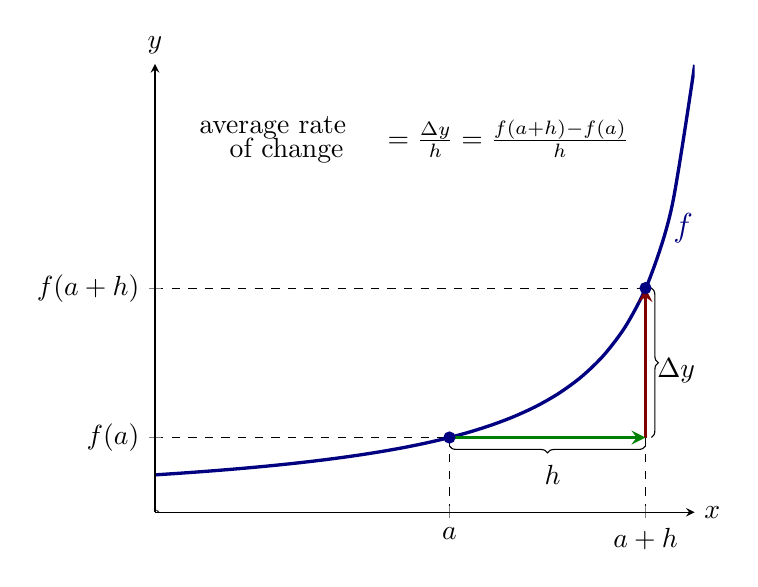
\begin{tikzpicture}
  \begin{axis}[
      domain=0:3, range=0:6,ymax=6,ymin=0,
      axis lines =left, xlabel=$x$, ylabel=$y$,
      every axis y label/.style={at=(current axis.above origin),anchor=south},
      every axis x label/.style={at=(current axis.right of origin),anchor=west},
            xtick={1,1.666}, ytick={1,3},
            xticklabels={$a$,$a+h$}, yticklabels={$f(a)$,$f(a+h)$},
            axis on top,
    ]         
         % \addplot [penColor2!15!background, domain=(0:2)] {-3.348+4.348*x};
        %  \addplot [penColor2!32!background, domain=(0:2)] {-2.704+3.704*x};
        %  \addplot [very thick,penColor2, domain=(0:2)] {-1.994+2.994*x};         
        %  \addplot [penColor2!66!background, domain=(0:2)] {-1.326+2.326*x}; 
         % \addplot [penColor2!83!background, domain=(0:2)] {-0.666+1.666*x};
	  \addplot [textColor,dashed] plot coordinates {(1,0) (1,1)};
          \addplot [textColor,dashed] plot coordinates {(0,1) (1,1)};
          \addplot [textColor,dashed] plot coordinates {(0,3) (1.666,3)};
          \addplot [textColor,dashed] plot coordinates {(1.666,0) (1.666,3)};
          \addplot [very thick,penColor, smooth,domain=(0:1.833)] {-1/(x-2)};
            \addplot[decoration={brace,mirror,raise=.06cm},decorate,thin] plot coordinates
                       {(1,0.95) (1.666,0.95)};
                         \addplot[decoration={brace,mirror,raise=.06cm},decorate,thin] plot coordinates
                       {(1.67,1) (1.67,3)};

          \addplot[color=penColor,fill=penColor,only marks,mark=*] coordinates{(1.666,3)};  %% closed hole          
          \addplot[color=penColor,fill=penColor,only marks,mark=*] coordinates{(1,1)};  %% closed hole          
         % \addplot [very thick,penColor2, smooth,domain=(0:2)] {x};
          \addplot [very thick,penColor2,->]  plot coordinates {(1.666,1) (1.666,3)};
             \addplot [very thick,penColor4,->]  plot coordinates {(1,1) (1.666,1)};
              \node at (axis cs:0,-0.1) {$0$};
               \node at (axis cs:1.35,0.5) {$h$ };
    
                \node at (axis cs:1.77,1.9) {$\Delta y$ };
                      \node at (axis cs:1.2,5) {$=\frac{\Delta y}{h}=\frac{f(a+h)-f(a)}{h}$ };
                       \node at (axis cs:0.4,5.15) {average rate};
                       \node at (axis cs:0.447,4.84){of change};
                        \node[color=penColor] at (axis cs:1.794,3.8){\large$f$};
        \end{axis}
\end{tikzpicture}
\end{image}
Now we can write
\[
{\text{average rate of change  }}=\frac{f(a+h)-f(a)}{(a+h)-a}=\frac{f(a+h)-f(a)}{h}
  \]
  What happens if $h\to0$? In other words, what is the meaning of the limit
\[
 \lim_{h\to 0} \frac{f(a+h)-f(a)}{h}?
\]
Obviously, this limit represents $f'(a)$, the instantaneous rate of change of $f$ at $a$! Therefore, 
we have 
an alternate way of writing the definition of the derivative at the point $a$, namely
\[
f'(a) = \lim_{h\to 0} \frac{f(a+h)-f(a)}{h}.
\]

\begin{example}
 Let $f(x) = x^2-2x$. Using the alternate expression for the derivative, find the slope of the tangent line to the curve $y=f(x)$ at the point $(2,f(2))$.
  \begin{explanation}
   The slope of the tangent line is given by the derivative, $f'(2)$.
    \[
    f'(2) =  \lim_{h\to 0}\frac{f\left(\answer[given]{2+h}\right)-f\left(2\right)}{h}.
    \]
    Now substitute in for the function we know,
    \[
    f'(2) = \lim_{h\to 0}\frac{(2+h)^2-2(2+h) -0}{h}.
    \]
    Now expand the numerator of the fraction,
    \[
     f'(2) =\lim_{h\to 0}  \frac{4+4h+h^2-4-2h }{h}.
    \]
    Now combine like-terms,
    \[
    f'(2) = \lim_{h\to 0} \frac{2h+h^2}{h}.
    \]
    Factor an $h$ from every term in the numerator,
    \[
   f'(2) =  \lim_{h\to 0}\frac{\cancel{h}\left(2+h\right)}{\cancel{h}}.
    \]
  Compute the limit,
    \[
     f'(2) =  \lim_{h\to 0}(2+h)=\answer[given]{2}. 
    \]
  \end{explanation}
\end{example}


	
This alternate definition of the derivative of $f$ at $a$, namely,


\[
f'(a) = \lim_{h\to 0}\frac{f(a+h)-f(a)}{h},
\]
(provided that the limit exists), allows us to define $f'(x)$ 
 for any value of $x$, 

\[
f'(x) = \lim_{h\to 0}\frac{f(x+h)-f(x)}{h},
\]
(provided that the limit exists).

And this is how we define a new function, $f'$, the derivative of $f$. The domain of $f'$ consists of all points in the domain of $f$ where the function $f$ is differentiable.
$f'(x)$ gives us the instantaneous rate of change of $f$ at any point $x$ in the domain of $f'$.\\
\begin{comment}
\begin{warning}
  The notation:
  \begin{quote}
  $f'(a)$ means take the derivative of $f$ first, then evaluate at
    $x=a$.
  \end{quote}
  In other words, given $f$ a function of $x$
  \[
  f'(a) = \eval{\ddx f(x)}_{x=a}.
  \]
\end{warning}
\end{comment}
Given a function $f$ from  some set of real numbers to the real numbers, the
derivative $f'$ is also a function from some set of real numbers to the real
numbers. Understanding the relationship between the \textit{functions}
$f$ and $f'$ helps us understand any situation (real or imagined)
involving changing values.
\begin{comment}
\begin{question}
  Let $f(x) = 3x+2$. What is $f'(-1)$?
  \begin{multipleChoice}
    \choice{$f'(-1) = 0$ because $f'(3)$ is a number, and a number corresponds to a horizontal line, which has a slope of zero.}
    \choice[correct]{$f'(-1) = 3$ because $y=f(x)$ is a line with slope $3$.}
    \choice{We cannot solve this problem yet.}
  \end{multipleChoice}
\end{question}
\end{comment}
\begin{example}
	Given the function $f(x) = 3x+2$, find  $f'(x)$. \\
	
	\begin{explanation}
		Start with the definition of $f'(x)$
		\[
		f'(x) = \lim_{h\to0}\frac{f(x+h)-f(\answer[given]{x})}{h}.
		\]
		Replace $f$ with its formula,
		\[
		f'(x) = \lim_{h\to0}\frac{3(x+h)+2-\left(\answer[given]{3x+2}\right)}{h}.
		\]
		Simplify the top,
		\[
		f'(x) = \lim_{h\to0}\frac{3\cancel{h}}{\cancel{h}}.
		\]
		Evaluate the limit.		
		\[
		f'(x) = \lim_{h\to0}{3}=\answer[given]{3}.
		\]

		
	\end{explanation}
\end{example}

\begin{example}
	Given the function $f(x) = |x|$, find  $f'(x)$. \\
	
	\begin{explanation}
	Recall, the  domain of $f$ is  $\RR$ and 
  $f$ is in fact a piecewise defined function, since
  \[
f(x) = |x|=
\begin{cases}
  \answer[given]{-x} &\text{if $x<0$,}\\
  \answer[given]{x} &\text{if $x\ge 0$}.
\end{cases}
\]
We will first compute $f'(x)$ when $x>0$.
		Start with the definition of $f'(x)$
		\[
		f'(x) = \lim_{h\to0}\frac{f(x+h)-f(\answer[given]{x})}{h}.
		\]
		Replace $f$ with its formula,
		\[
		f'(x) = \lim_{h\to0}\frac{|x+h|-\answer[given]{|x|}}{h}.
		\]
		\[
		f'(x) = \lim_{h\to0}\frac{x+h-\answer[given]{x}}{h}.
		\]
		Note: When $x>0$, then for all small enough values of  $h$ it follows that $x+h>0$. 
		Therefore, $|x+h|=x+h$.
		Now we have
		\[
		f'(x) = \lim_{h\to0}\frac{h}{h}= \lim_{h\to0}\answer[given]{1}=\answer[given]{1}.
		\]
	Now, we can compute the derivative 	$f'(x)$ when $x<0$.
\[
		f'(x) = \lim_{h\to0}\frac{f(x+h)-f(\answer[given]{x})}{h}.
		\]
		Replace $f$ with its formula,
		\[
		f'(x) = \lim_{h\to0}\frac{|x+h|-\answer[given]{|x|}}{h}.
		\]
		\[
		f'(x) = \lim_{h\to0}\frac{-x-h-\answer[given]{-x}}{h}.
		\]
		Note: When $x<0$, then for all small enough values of  $h$ it follows that $x+h<0$. 
		Therefore, $|x+h|=-(x+h)=-x-h$.
		Now we have
		\[
		f'(x) = \lim_{h\to0}\frac{-h}{h}= \lim_{h\to0}\answer[given]{-1}=\answer[given]{-1}.
		\]
		What remains to be done is to check whether the derivative $f'(0)$ exists.
		Start with the definition of $f'(0)$
		\[
		f'(0) = \lim_{h\to0}\frac{f(0+h)-f(\answer[given]{0})}{h}.
		\]
		Replace $f$ with its formula,
		\[
		f'(0) = \lim_{h\to0}\frac{|0+h|-\answer[given]{|0|}}{h}.
		\]
		\[
		f'(0) = \lim_{h\to0}\frac{|h|}{h}.
		\]
		Note: When $h>0$, then $|h|=h$, but when $h<0$, then $|h|=-h$. 
		Therefore, instead of computing the limit above, we will compute the two one-sided limits and compare them.
		
		\[
		 \lim_{h\to0^+}\frac{|h|}{h}= \lim_{h\to0^+}\frac{h}{h}=\lim_{h\to0^+}\answer[given]{1}=\answer[given]{1};
		\]
		\[
		 \lim_{h\to0^-}\frac{|h|}{h}= \lim_{h\to0^-}\frac{-h}{h}=\lim_{h\to0^-}\answer[given]{-1}=\answer[given]{-1};
		\]
		Since the two one-sided limits are not equal it follows that 
		\[
		 \lim_{h\to0}\frac{|h|}{h} {\text{           DOES NOT EXIST!}}
		\]
		Therefore,   $f'(0)$ DOES NOT EXIST, which means that $f$ is NOT DIFFERENTIABLE at $x=0$!
		To summarize
		
		 \[
f'(x) =
\begin{cases}
  \answer[given]{-1} &\text{if $x<0$,}\\
  \answer[given]{1} &\text{if $x> 0$}.
\end{cases}
\]
	\end{explanation}
\end{example}

\begin{question}
  Is it true that for any function $f$ the domain of $f'$ is equal to the domain of $f$?
  \begin{prompt}
  \begin{multipleChoice}
    \choice{yes}
    \choice[correct]{no}
  \end{multipleChoice}
  \begin{feedback}
  This is not true. 
  Consider the function $f(x)=|x|$. 
The domain of $f$ is $\RR$ and the domain of $f'$ is $(-\infty,0)\cup(0,\infty)$


This example demonstrates that a function $f$ and its derivative, $f'$, may have different domains.
  \end{feedback}
  \end{prompt}
\end{question}

\begin{question}
  Can two different functions, say, $f$ and $g$, have the same derivative?
  \begin{prompt}
  \begin{multipleChoice}
    \choice[correct]{yes}
    \choice{no}
  \end{multipleChoice}
  \begin{feedback}
    Many different functions can share the same derivatives.
    Consider two different functions, $f$ and $g$, defined by\\
    $f(x)=x$ and $g(x)=x+5$.
    Then, $f'(x)=1$, and $g'(x)=1$, for all real numbers $x$.\\
    So,  the derivatives of these two different functions are equal.

  \end{feedback}
  \end{prompt}
\end{question}

Let's compare the graphs of $f$ and $f'$ for the derivatives we've computed so far:

\[f(x)=x^2, f'(x)=2x\]
\begin{image}
    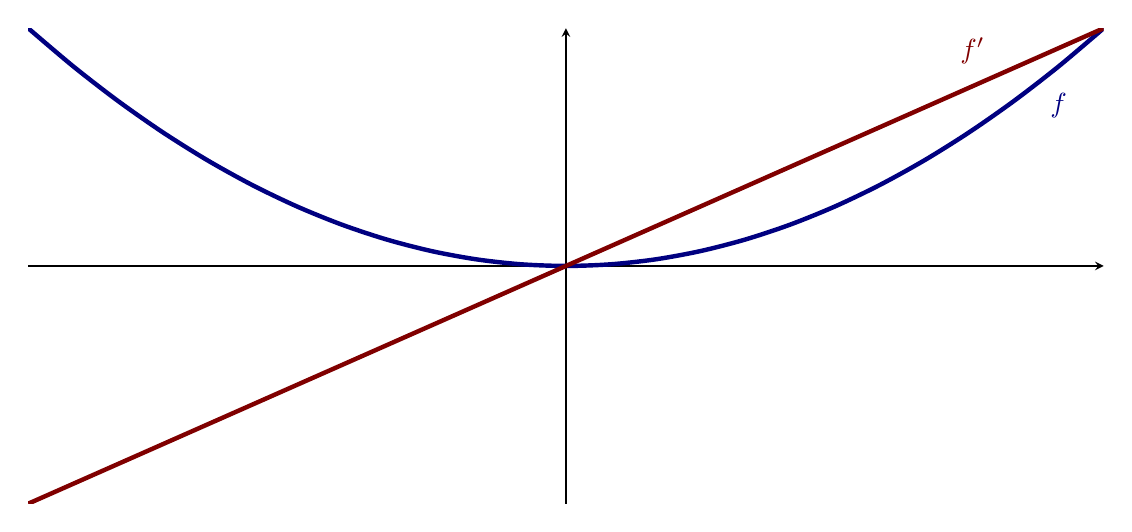
\begin{tikzpicture}
      \begin{axis}[
          xmin=-2,xmax=2,ymin=-4,ymax=4,
          axis lines=center,
          ticks=none,
          width=6in,
          height=3in,
          every axis y label/.style={at=(current axis.above origin),anchor=south},
          every axis x label/.style={at=(current axis.right of origin),anchor=west},
        ]
        %\addplot [ultra thick,dashed, penColor,smooth, domain=(-2:2)] {x^3+.3*x^2-2*x)};
        \addplot [ultra thick,penColor,smooth, domain=(-2:2)] {x^2} node [pos=0.9, below right] {$f$};
        \addplot [ultra thick,penColor2,smooth, domain=(-2:2)] {2*x} node [pos=0.9, above left] {$f'$};
      \end{axis}
    \end{tikzpicture}
  \end{image}

\[f(x)=3x+2, f'(x)=3\]
\begin{image}
    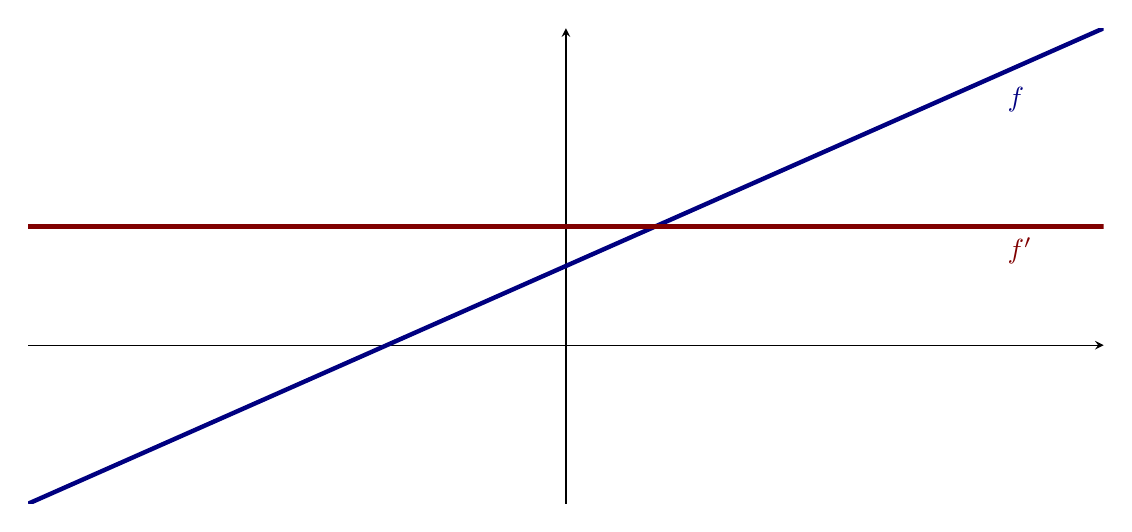
\begin{tikzpicture}
      \begin{axis}[
          xmin=-2,xmax=2,ymin=-4,ymax=8,
          axis lines=center,
          ticks=none,
          width=6in,
          height=3in,
          every axis y label/.style={at=(current axis.above origin),anchor=south},
          every axis x label/.style={at=(current axis.right of origin),anchor=west},
        ]
        %\addplot [ultra thick,dashed, penColor,smooth, domain=(-2:2)] {x^3+.3*x^2-2*x)};
        \addplot [ultra thick,penColor,smooth, domain=(-2:2)] {3*x+2} node [pos=0.9, below right] {$f$};
        \addplot [ultra thick,penColor2,smooth, domain=(-2:2)] {3} node [pos=0.9, below right] {$f'$};

      \end{axis}
    \end{tikzpicture}
  \end{image}

  % (su18:TK) fixed an error below
  % $$f(x)=|x|, f'(x)=\begin{cases} 1 &  \text{for } x<0 \\ -1 &
  %   \text{for } x>0 \end{cases}$$ %fliiped signs
  \[f(x)=|x|, f'(x)=\begin{cases} 1 &  \text{for } x>0 \\ -1 & \text{for } x<0 \end{cases}\]

  \begin{image}
    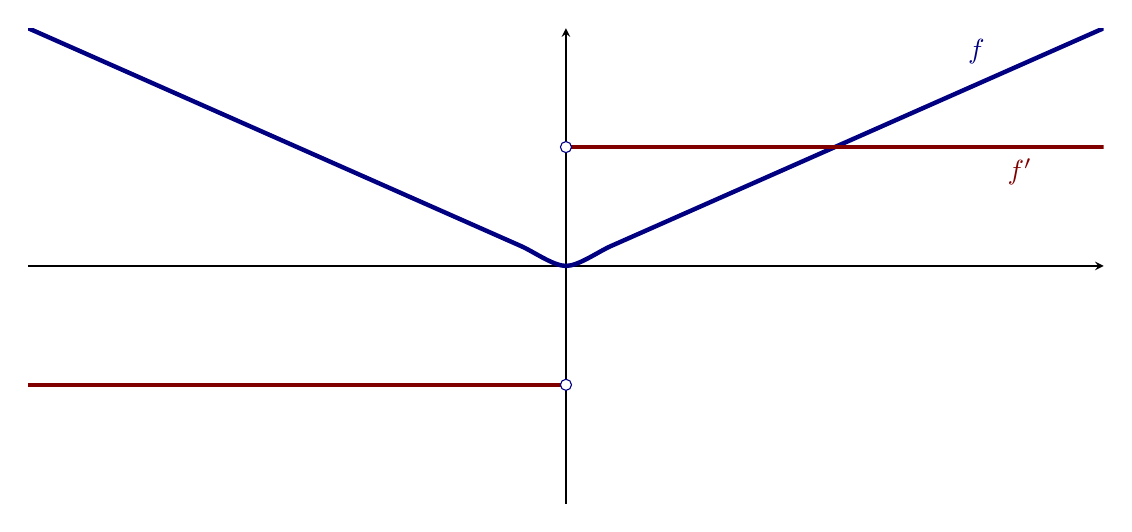
\begin{tikzpicture}
      \begin{axis}[
          xmin=-2,xmax=2,ymin=-2,ymax=2,
          axis lines=center,
          ticks=none,
          width=6in,
          height=3in,
          every axis y label/.style={at=(current axis.above origin),anchor=south},
          every axis x label/.style={at=(current axis.right of origin),anchor=west},
        ]
        %\addplot [ultra thick,dashed, penColor,smooth, domain=(-2:2)] {x^3+.3*x^2-2*x)};
        \addplot [ultra thick,penColor,smooth, domain=(-2:2)] {abs(x)} node [pos=0.9, above left] {$f$};
        \addplot [ultra thick,penColor2,smooth, domain=(-2:0)] {-1};
        \addplot [ultra thick,penColor2,smooth, domain=(0:2)] {1} node [pos=0.8, below right] {$f'$};
        \addplot[color=penColor,fill=background,only marks,mark=*] coordinates{(0,-1)};
        \addplot[color=penColor,fill=background,only marks,mark=*] coordinates{(0,1)};
      \end{axis}
    \end{tikzpicture}
  \end{image}
  \begin{question}
 For each of the three pairs of functions, describe $y=f(x)$ when $f'$
  is positive, and when $f'$  is negative.\\

  \begin{prompt}
    When $f'$ is positive, $y=f(x)$ is \wordChoice{\choice{positive}\choice[correct]{increasing}\choice{negative}\choice{decreasing}}.
    When $f'$ is negative, $y=f(x)$ is \wordChoice{\choice{positive}\choice{increasing}\choice{negative}\choice[correct]{decreasing}}
  \end{prompt}
      \end{question}
\begin{question}
  Here we see the graph of $f'$, the derivative of some function $f$.
  \begin{image}
    \begin{tikzpicture}
      \begin{axis}[
          xmin=-2,xmax=2,ymin=-8,ymax=8,
          axis lines=center,
          ticks=none,
          width=6in,
          height=3in,
          every axis y label/.style={at=(current axis.above origin),anchor=south},
          every axis x label/.style={at=(current axis.right of origin),anchor=west},
        ]
        %\addplot [ultra thick,dashed, penColor,smooth, domain=(-2:2)] {x^3+.3*x^2-2*x)};
        \addplot [ultra thick,penColor,smooth, domain=(-2:2)] {3*x^2+2*.3*x-2)};
      \end{axis}
    \end{tikzpicture}
  \end{image}


    Which of the following graphs could be $y = f(x)$?
     \begin{multipleChoice}
       \choice{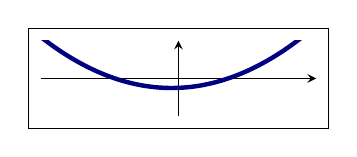
\begin{tikzpicture}[framed,scale=1,baseline=3ex]
           \begin{axis}[
               xmin=-2,xmax=2,ymin=-8,ymax=8,
               axis lines=center,
               ticks=none,
               width=2in,
               height=1in,
               every axis y label/.style={at=(current axis.above origin),anchor=south},
               every axis x label/.style={at=(current axis.right of origin),anchor=west},
             ]
             \addplot [ultra thick,penColor,smooth, domain=(-2:2)] {3*x^2+2*.3*x-2)};
           \end{axis}
       \end{tikzpicture}}
       \choice[correct]{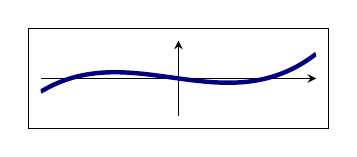
\begin{tikzpicture}[framed,scale=1,baseline=3ex]
           \begin{axis}[
               xmin=-2,xmax=2,ymin=-8,ymax=8,
               axis lines=center,
               ticks=none,
               width=2in,
               height=1in,
               every axis y label/.style={at=(current axis.above origin),anchor=south},
               every axis x label/.style={at=(current axis.right of origin),anchor=west},
             ]
             \addplot [ultra thick,penColor,smooth, domain=(-2:2)] {x^3+.3*x^2-2*x)};
           \end{axis}
       \end{tikzpicture}}
       \choice{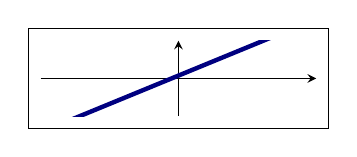
\begin{tikzpicture}[framed,scale=1,baseline=3ex]
           \begin{axis}[
               xmin=-2,xmax=2,ymin=-8,ymax=8,
               axis lines=center,
               ticks=none,
               width=2in,
               height=1in,
               every axis y label/.style={at=(current axis.above origin),anchor=south},
               every axis x label/.style={at=(current axis.right of origin),anchor=west},
             ]
             \addplot [ultra thick,penColor,smooth, domain=(-2:2)] {6*x+2*.3)};
           \end{axis}
       \end{tikzpicture}}
     \end{multipleChoice}

\end{question}
\begin{comment} 
\begin{question} 
    Which of the following computes the derivative, $f'(a)$?
    \begin{selectAll}
      \choice{$\lim_{h\to 0}\frac{(f(a)+h) - f(a)}{(a+h)-a}$}
      \choice[correct]{$\lim_{h\to 0}\frac{f(a+h) - f(a)}{(a+h)-a}$}
      \choice{$\lim_{h\to 0}\frac{(f(a)-h) - f(a)}{(a-h)-a}$}
      \choice[correct]{$\lim_{h\to 0}\frac{f(a-h) - f(a)}{(a-h)-a}$}
      \choice{$\lim_{h\to 0}\frac{f(a) - (f(a)+h)}{a-(a+h)}$}
      \choice[correct]{$\lim_{h\to 0}\frac{f(a) - f(a+h)}{a-(a+h)}$}
      \choice{$\lim_{h\to 0}\frac{f(a) - (f(a)-h)}{a-(a-h)}$}
      \choice[correct]{$\lim_{h\to 0}\frac{f(a) - f(a-h)}{a-(a-h)}$}
    \end{selectAll}
\end{question}	
\end{comment} 
\end{document}
